\section{Overview and Background}\label{sec:big-picture}

\subsection{Game Types}
%TODO: needs a better word than types, more like architectures. Feedback welcome
Describe different types of games, i.e. local games, client-server games, streamed games.

% TODO: We could use one figure with three subfigures which shows the (ever increasing)
%       number of components 

\paragraph*{Local Games}

\paragraph*{Client-Server Games}

\paragraph*{Streaming Games}

At the end of this subsection, the reader should understand which (technological) components make up the different types of games.

\subsection{Big Picture}

This subsection adds the player to the architectures introduced above, highlights potential QoS and QoE (or discusses why some chosing a particular QoE metric is not useful) metrics to study.

\begin{figure}
  \centering
  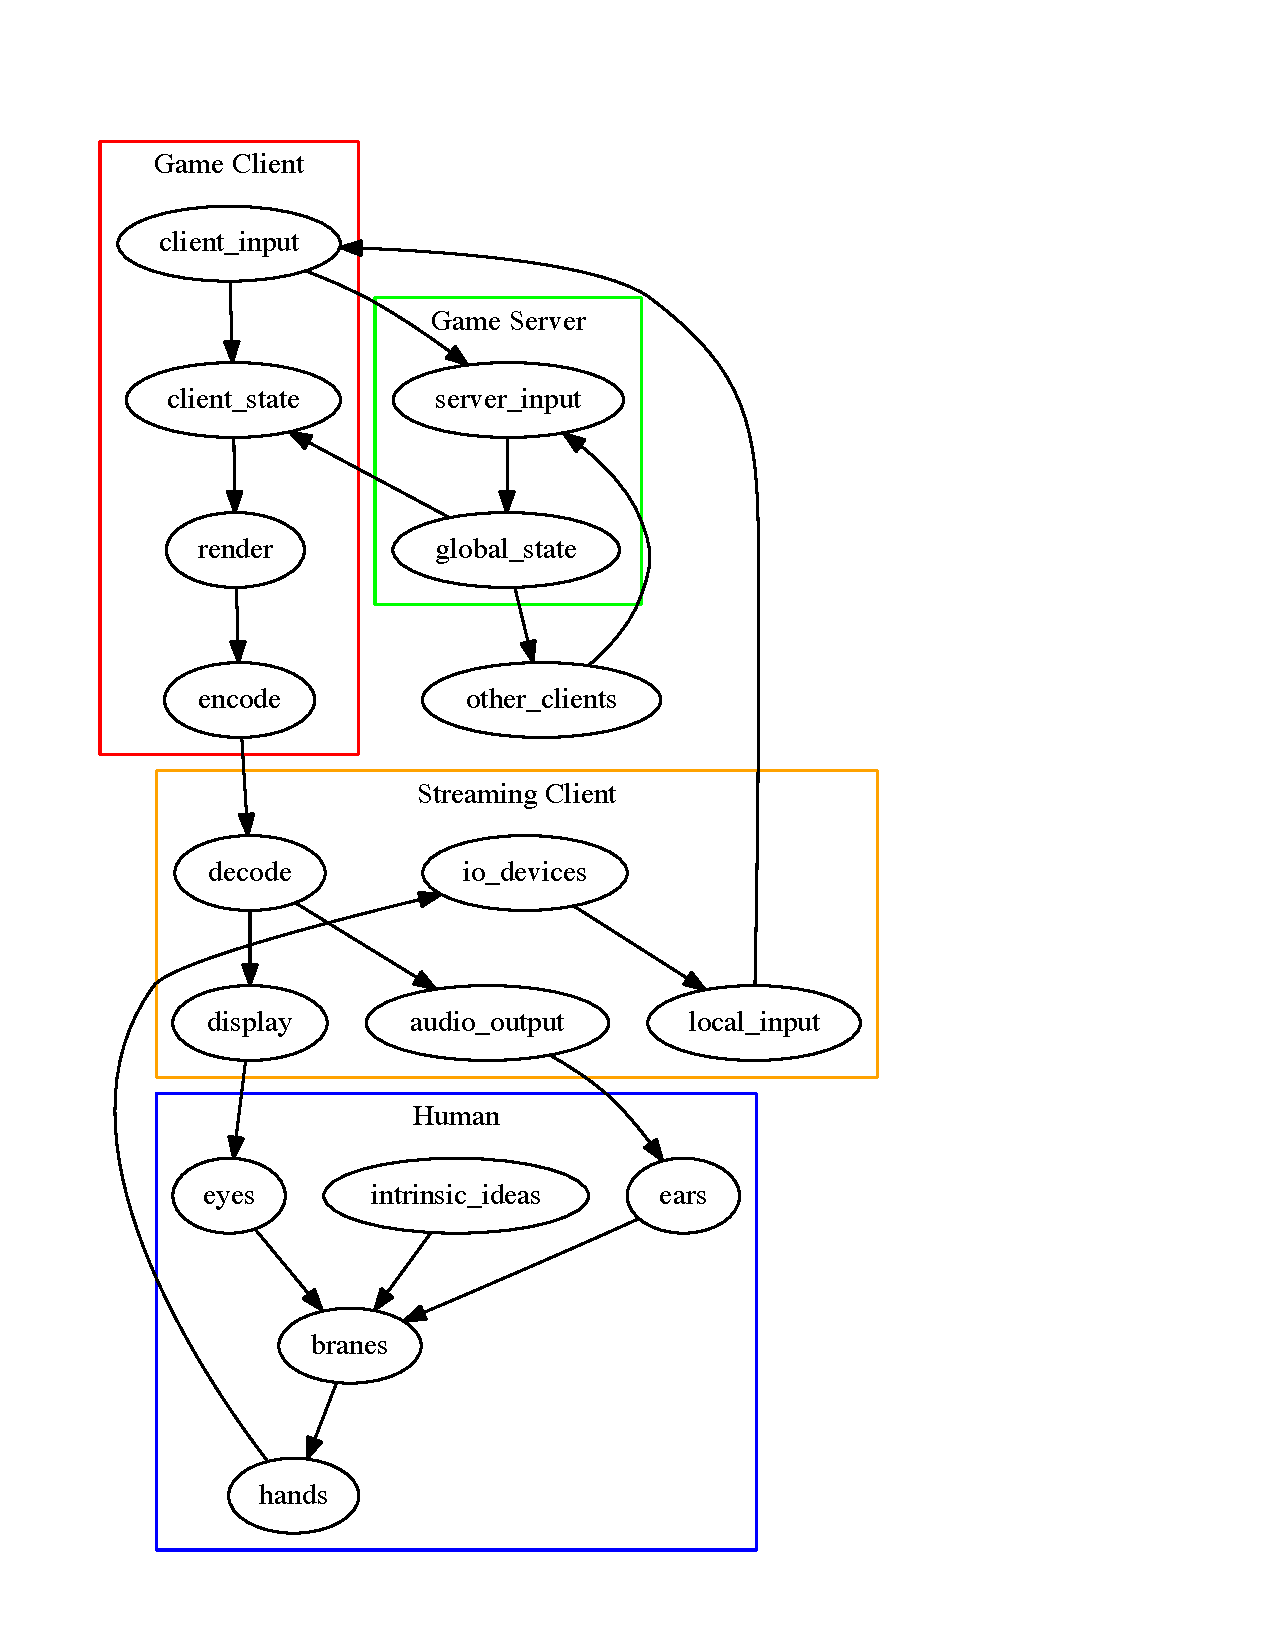
\includegraphics[width=1.0\columnwidth]{../models/cycle.pdf}
  \caption{Interaction of TODO.}
  \label{fig:component-model}
\end{figure}

At the end of this section, the reader should agree that end to end latency is a sensible starting point to study video game qos.